% exercise sheet with header on every page for math or close subjects
\documentclass[12pt]{article}
\usepackage[utf8]{inputenc}
\usepackage{latexsym}
\usepackage{multicol}
\usepackage{fancyhdr}
\usepackage{amsfonts}
\usepackage{amsmath}
\usepackage{amssymb}
\usepackage{enumerate}
\usepackage{listings}
\usepackage{graphicx}
\usepackage{amssymb}

% Shortcuts for bb, frak and cal letters
\newcommand{\E}{\mathbb{E}}
\newcommand{\V}{\mathbb{V}}
\renewcommand{\P}{\mathbb{P}}
\newcommand{\N}{\mathbb{N}}
\newcommand{\R}{\mathbb{R}}
\newcommand{\C}{\mathbb{C}}
\newcommand{\Z}{\mathbb{Z}}
\newcommand{\Pfrak}{\mathfrak{P}}
\newcommand{\Pfrac}{\mathfrak{P}}
\newcommand{\Bfrac}{\mathfrak{P}}
\newcommand{\Bfrak}{\mathfrak{B}}
\newcommand{\Fcal}{\mathcal{F}}
\newcommand{\Ycal}{\mathcal{Y}}
\newcommand{\Bcal}{\mathcal{B}}
\newcommand{\Acal}{\mathcal{A}}

% formating
\topmargin -3.5cm
\textheight 22cm
\textwidth 16.0 cm
\oddsidemargin -0.1cm

% Fancy Header on every Page
\pagestyle{fancy}
\lhead{\textbf{Embedded Systems Milestone 6}}
\rhead{Rafael Dewes (2548365) \\ Kevin M\"uller (2550062) \\ Daniel Schäfer (2549458)\\ }
\renewcommand{\headrulewidth}{1.2pt}
\setlength{\headheight}{110pt}

\begin{document}
\pagenumbering{gobble}
\lstset{language=C++}

\section*{Test Series}
\subsection*{Line Sensor Readings}
We tested the line sensors in different lighting environments and for multiple line colours.


\begin{tabular}{ | l | r | r | r | r | }
\hline
Lighting & Readings for & & & \\
Conditions & White ground & Blue line & Grey line & Black line \\ \hline
Bright & 0000 & 0000 & 0000 & 0000 \\ \hline
Medium & 0000 & 0000 & 0000 & 0000 \\ \hline
Dark & 0000 & 0000 & 0000 & 0000 \\
\hline
\end{tabular}

\subsection*{Velocity vs. Line Count}
The following table contains our results from testing the accuracy of the motor velocity against the lines our line sensors counted.


\begin{tabular}{ | c || r | r | r | r | }
\hline
Real distance & Velocity & Line Count & $\delta$Velocity & $\delta$Lines \\
 ( x, y) & & & & \\ \hline
10, 0 & 9.8,0 & 1,0 & 0.2 & 0 \\ \hline
15, 0 & 14.3,0 & 1,0 & 0.7 & 5 \\ \hline
15, 0 & 14.3,0 & 1,0 & 0.7 & 5 \\ \hline
15, 0 & 14.3,0 & 1,0 & 0.7 & 5 \\ \hline
15, 0 & 14.3,0 & 1,0 & 0.7 & 5 \\ \hline
15, 0 & 14.3,0 & 1,0 & 0.7 & 5 \\ \hline
\end{tabular}

\subsection*{Velocity vs. Referee Updates}
Accuracy of the position updates sent by the referee versus the interpolation of our position with motor velocity.


\begin{tabular}{ | c || r | r | r | r | }
\hline
Real distance & Velocity & Pos Update & $\delta$Velocity & $\delta$Pos Update \\
 ( x, y) & & & & \\ \hline
10, 0 & 9.8,0 & 10,0 & 0.2 & 0 \\ \hline
15, 0 & 14.3,0 & 10,0 & 0.7 & 5 \\ \hline
15, 0 & 14.3,0 & 10,0 & 0.7 & 5 \\ \hline
15, 0 & 14.3,0 & 15,0 & 0.7 & 5 \\ \hline
15, 0 & 14.3,0 & 15,0 & 0.7 & 5 \\ \hline
15, 0 & 14.3,0 & 15,0 & 0.7 & 5 \\ \hline
\end{tabular}

\section*{Testing Against a Model}

\subsection*{Timed Automaton}
\begin{center}


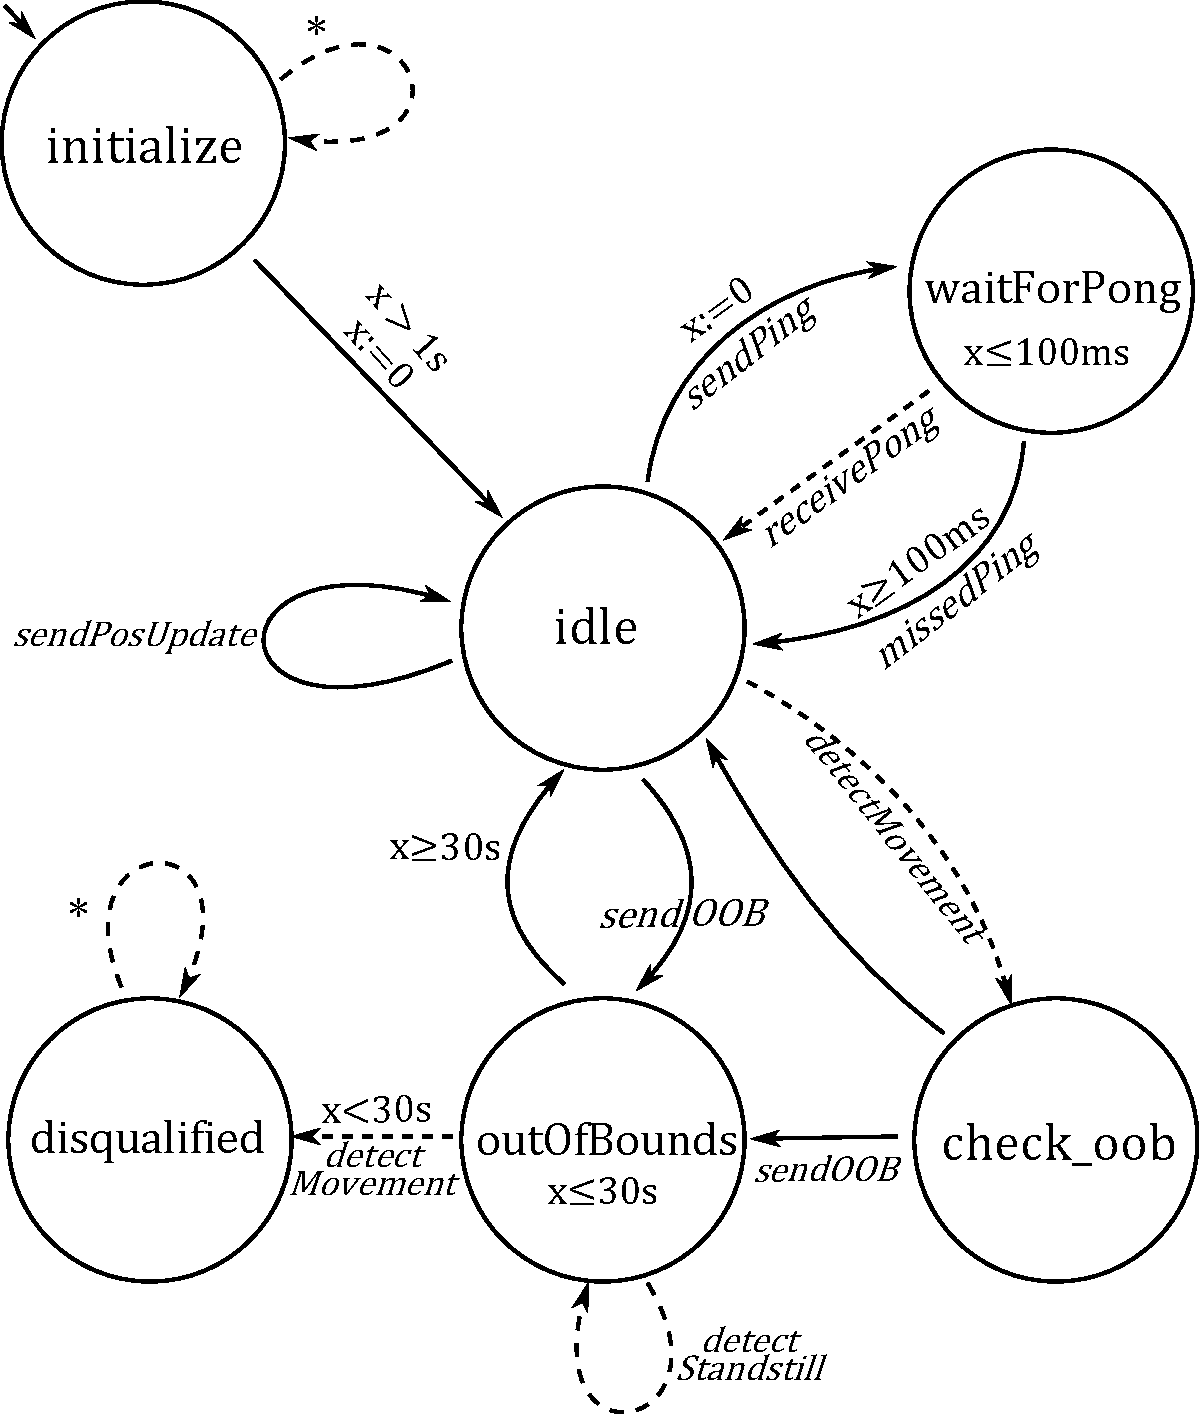
\includegraphics[width = 0.75\textwidth]{images/ref_ta.pdf}

Timed automaton representing the referee.

\end{center}

\subsection*{Testing Runs}
We have one run to test the robot's reaction to ping:
\[ \tau \rightarrow (sendPing \rightarrow \tau \rightarrow receivePong)^{*}  \] 

\flushleft
The second run secures that the robot reacts correctly to an Out-of-bounds message:
\[ \tau \rightarrow sendPosUpdate\rightarrow sendOOB \rightarrow (detectStandstill | \tau )^{*} \rightarrow penaltyOver \rightarrow \dots \]

\subsection*{Implementation and Changes}
To model the nondeterminism we introduced a random variable into the simulation. Pings are sent at irregular intervals, and wait times after every transition are randomized.
\end{document}

